\documentclass[a4paper]{article}

%Packages
\usepackage[swedish]{babel}
\usepackage[T1]{fontenc}
\usepackage[utf8]{inputenc}
\usepackage{graphicx}
\usepackage{float}

\newcommand\namn{Larmsystem}

\restylefloat{table}

\begin{document}

%
% Front page
%

\thispagestyle{empty}

\begin{center}
    \parskip=14pt%
    \vspace*{3\parskip}%

    {\LARGE Projektplan DAT290}

    {\large \namn, grupp 11

    Titus Blosse, Viktor Frideen, Nazif Kadiroglu, Markus Moen, Lukas Schiavone, Fredrik Österström

    \today}

    \rule{7cm}{0.4pt}\\
\end{center}
\newpage

%
% ToC, Table of Contents 
%

\thispagestyle{empty}

\tableofcontents
\newpage

%
% Projektplan
%

\pagenumbering{arabic}

\section{Syfte}

År 2019 anmäldes 75250  inbrottsstölder i Sverige vilket är en minskning med 14\%\ från året innan \cite{brastold}. Detta är en stark minskning och en trend som vi gärna ser fortsätta gå åt samma håll. Därför har vi valt att utveckla ett larm som enkelt kan installeras i alla typer av bostäder och som ger ett grundligt skydd mot oönskat intrång. Vi eftersträvar att i den slutgiltiga produkten kunna erbjuda en rad olika larmkomponenter som enkelt kan anslutas till en larmcentral och konfigureras för att passa kundens specifika sitution.

%Detta syfte kanske är lite för bakgrundigt?

\section{Mål}

Vi strävar efter att utveckla ett system som ska ge användaren bättre kontroll och övervakningsmöjligheter över sina tillhörigheter. Systemet ska vara väldokumenterat och fackmannamässigt utfört med goda förutsättningar för expansion. Grunden i systemet kommer vara en centralenhet till vilken användaren kan ansluta olika periferienheter. Huvudsakligen kommer två periferienheter att utecklas, ett dörrlarm samt ett rörelselarm.

%Fylla på lite här om vi ska göra några extrauppgifter?
%Vi bör granska ord som personaliserar texten, ex: Vi, jag etc. Går dessa att undvika i sammahanget?

\section{Bakgrund}

\subsection{Begrepp}

\begin{description}
    \item[CAN:] Controller Area Network
    \item[MD407:] Mikrodator av typen MD407 
\end{description}

\subsection{Referenser}

\subsection{Tekniska förutsättningar}

Hårdvaran för att driva larmsystemet är färdigutvecklad och dokumenterad. Tre mikro-datorer av typen MD407 driver tillsammans periferienheterna och centralenheten. För kommunikation mellan datorerna via CAN-bussen finns ett kodexempel. Periferienheterna använder sig av sensorer för att upptäcka och initiera ett alarm som skickas till centralenheten. Till varje periferienhet kopplas en sensor av typen dörr-, vibrations- och avståndssensor. Detta möjliggör 3 över 2 olika kombinationer av sensorer med periferienheterna.

\section{Systemöversikt}

\begin{figure}[H]
    \centering
    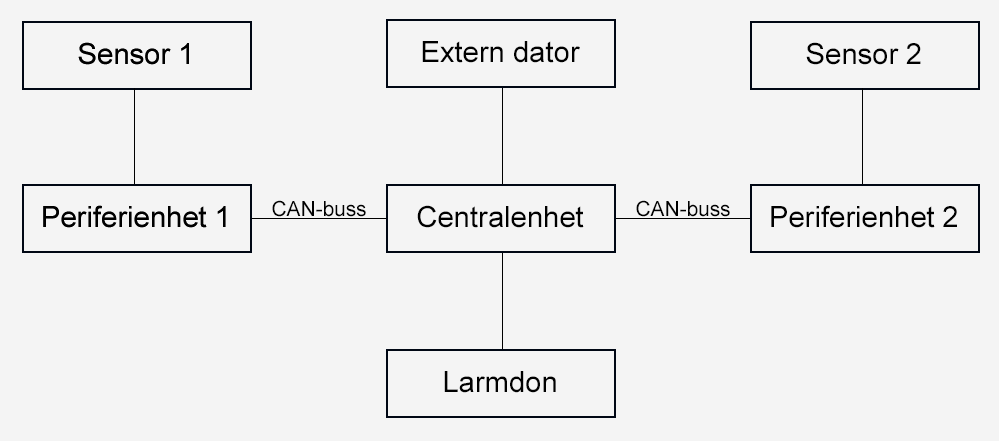
\includegraphics[width=\textwidth]{blockschema.png}
    \caption{Blocksschema över larmsystemet}
    %\label{fig:my_label}
\end{figure}

Centralenheten kommunicerar med periferienheterna genom en \textit{Controller Area Network}-buss. Periferienheterna undersöker ändringar hos deras sensorer och vid funnen ändring rapporteras detta till centralenheten för larm. Inrapporteringen sker via ett meddelande på bussen som skapar ett avbrott hos centralenheten och aktiverar larmdonet.

Centralenheten måste kunna identifiera vilken periferienhet som skickat meddelandet och förstå varför det skicades. Centralenhetenen kommunicerar med en dator för att ge användaren en tydlig bild om var larmet uppstod.

\section{Resursplan}

I följande lista finns e-mailadresser till gruppens medlemmar, men för intern kommunikation används både Discord och Messenger. Gruppmöten kommer i första hand a ske igenom Zoom.

Ansvar i följande lista syftar inte till att en ansvarig skall göra allt inom sitt ansvarsområde, utan till att den ansvarige ska se till att det sköts ordentligt utav hela gruppen.

\begin{description}
    \item[Titus Blosse, administrativt dokumentansvarig:] Ansvarar för att mötesprotokoll förs och att de olika rapporterna som ska skrivas under projektets gång såväl påbörjas som skickas in i tid.

    E-mail: titus.blosse@gmail.com

    \item[Viktor Frideen, planeringsansvarig:] Ansvarar för att informera gruppen om hur arbete med projektet och dess delmål fortgår och även för att uppmärksamma gruppen om de hamnar efter planeringen.

    E-mail: viktor.frideen@outlook.com

    \item[Nazif Kadiroglu, teknik dokumentansvarig:] Ansvarar för att all kod i projektet är väl dokumenterad.

    E-mail:

    \item[Markus Moen, testansvarig:] Ansvarar för att tester på både hårdvara och mjukvara testas och dokumenteras väl.

    E-mail: markus.offersten@gmail.com

    \item[Lukas Schiavone, kodansvarig:] Ansvarar för att gruppen följer den kodstandard de har satt.

    E-mail: luksch1121@gmail.com

    \item[Fredrik Österström, gruppledare och resursansvarig:] Ansvarar för att kommunikation med kursens lärare, gruppmöten, hårdvarans tillgänglighet och att de verktyg gruppen har valt för kommunikation och versionhantering används väl.

    E-mail:
\end{description}

Hårdvaran för detta projekt finns tillgänglig i rum 4209 i EDIT-huset på Chalmers campus. Detta rum, och med det hårdvaran, kan bokas via en anslagstavla som även den finns i EDIT-huset. Det är dock möjligt att anslagstavlan kommer bytas ut till ett digitalt alternativ. Hårdvaran som finns tillgänglig är:

\begin{itemize}
    \item 3x MD407 kort
    \item 1x Avståndsmätare (ultraljud), HC-SR04
    \item 1x Vibrationssensor, "Flying-Fish" SW-18010P
    \item 1x Keypad
    \item 1x 7-segmentsdisplay
    \item 2x 4-polig RJ-11 kabel (används för CAN-bussen)
    \item 1x RJ-11 förgrening
    \item 2x Tiopolig flatkabel
    \item 3x USB-kabel
    \item 1x Kopplingsplatta
\end{itemize}

Mjukvaran som kommer användas är CodeLite vilket är fördelaktigt då den kan simulera MD407 korten och då gruppmedlemmarna har erfarenthet med denna mjukvara. GitHub används för versionshantering.

Mycket av arbetet kan ske på distans då endast test på hårdvaran kräver att gruppmedlemmar är på plats i Chalmers. För arbete på distans kan gruppen kommunicera via Discord, som stödjer både röst- och textbaserad kommunikation.

\section{Milstolpar}
Schiavone

\begin{table}[H]
    \begin{center}
        \begin{tabular}{ |c|c|c|c| }\hline
            Nr & Beskrivning & Datum \\\hline\hline
            %\multirow{3}{4em}{Multiple row} & cell2 & cell3 \\
            1 & Projektplan inlämnad & 2020-xx-xx \\\hline
            .. & ... & ... \\\hline
            .. & ... & ... \\\hline
            .. & ... & ... \\\hline
        \end{tabular}
        % Text underneath the table
        \caption{Milstolpar för projektet}
        % Label for reference usage
        \label{milstolpar}
    \end{center}
\end{table}

\section{Aktiviteter}

Gruppmedlemmarna förväntas spendera 200h vardera med ett totalt antal mantimmar motsvarande 1200h. De 200h som varje medlem i gruppen förväntas lägga ner innefattar all tid som spenderas under projektets gång.

\begin{table}[H]
    \begin{center}
        \begin{tabular}{ |c|c|c| }\hline
            Nr & Beskrivning & Tidsåtgång \\\hline\hline
            1 & Föreläsningar (4h/vecka, 8 veckor, 6 personer) & 192h \\\hline
            2 & Projektmöten (2h/vecka, 8 veckor, 6 personer) & 96h \\\hline
            3 & Skrivande av protocoll, kallelser etc & 20h \\\hline
            4 & Framtagning av LaTeX-mallar & 18h \\\hline
            5 & Arbeta med projektplan & 120h \\\hline
            6 & Dokumentations läsning & 50h \\\hline
            7 & Rapportutkast & 110h \\\hline
            8 & Renskrivande av Rapportutkast 1 & 15h \\\hline
            9 & Rapportutkast 2 & 70h\\\hline
            10 & Renskrivning ac rapportutkast 2 & 10h \\\hline
            11 & Oppositionsrapport & 30h\\\hline
            12 & Slutföring av projektrapport & 100h\\\hline
            13 & Programmering av periferienhet, dörr & 30h \\\hline
            14 & Programmering av periferienhet, rörelse & 30h \\\hline
            15 & Programmering av centralenhet & 50h \\\hline
            16 & Tester och testrapport & 100h\\\hline
            17 & Granskning av kod & 50h \\\hline
            18 & Teknisk dokumentation & 50 \\\hline
            19 & Förbered/genomför demonstration & 35h \\\hline
        \end{tabular}
        \caption{Aktivitetslista för projektet}
        \label{aktivitetslista}
    \end{center}
\end{table}

Projektet har delats upp i aktiviteter. Anledningen till detta är för att gruppen ska ha bättre koll på vad som ska genomföras under projektets gång och även optimal planering av nedlagda timmar. Viktigt att notera är att aktiviteterna har givits en uppskattad tidsåtgång i tabell \ref{aktivitetslista}. Tidsåtgången kan däremot variera under projektets gång där vissa aktiviteter kan kräva mer eller mindre tid än den upskattade tidsåtgången.





\section{Tidsplan}

\section{Mötesplan}

Mötestillfällen där alla gruppmedlemmar inklusive mentor medverkar.

\begin{table}[H]
    \begin{center}
        \begin{tabular}{ |c|c|c| }\hline
            Datum & tid & Lokal \\\hline\hline
            02/09-20 & 13:00-15:00 & ED4209 \\\hline
            09/09-20 & 15:00-17:00 & Zoom \\\hline
            16/09-20 & 13:00-15:00 & Zoom \\\hline
            23/09-20 & 13:00-15:00 & Zoom \\\hline
            30/09-20 & 13:00-15:00 & Zoom \\\hline
            07/10-20 & 13:00-15:00 & Zoom \\\hline
            14/10-20 & 13:00-15:00 & Zoom \\\hline
            21/10-20 & 13:00-15:00 & Zoom \\\hline
        \end{tabular}
        \caption{Tabell över mötestillfällen}
        \label{motesplan}
    \end{center}
\end{table}

\section{Kommunikationsplan}

\section{Kvalitetsplan}

\section{Spelregler}

% Tells the compiler what reference system to use
\bibliographystyle{ieeetr}
% Prints the reference list at the end of the file
\bibliography{referenser.bib}

\end{document}
